\documentclass[onlytextwidth]{beamer}
\usepackage[utf8]{inputenc}
\usepackage{microtype}
\usepackage{amsmath}
\usepackage{amssymb}
\usepackage[nomessages]{fp} %\FPeval{\var-name}{2*sin(pi/6)}
\usepackage{siunitx} %units in math. eg 20\milli\meter
\usepackage{yhmath} % for arcs, overparenth command
\usepackage{tikz} %graphics
\usetikzlibrary{quotes, angles}
%\usepackage{graphicx} already loaded by beamer class
%consider setting \graphicspath{{images/}}
%\parskip ?? to avoid paragraph indent
\usepackage{multicol} %may not need this package, just columns environment
\usepackage{venndiagram}

\subtitle[BECA]{Bronx Early College Academy}
\author[Huson]{Christopher J. Huson PhD}

\setbeamertemplate{headline}{\vskip2mm 
  BECA / \insertshortauthor \, / \inserttitle
  \hfill 
  \insertsection
  }

\title{Geometry Unit 3: Misc bank of slides}
\date{11 October - 21 October 2022}

\begin{document}
\frame{\titlepage}
\section[Outline]{}
\frame{\tableofcontents}

\section{Isosceles triangles}
\begin{frame}{The isosceles base angle theorem.}
  Given $\triangle ABC$. $\overline{AC} \cong \overline{BC}$ \emph{iff} $\angle A \cong \angle B$.\\[0.5cm]
  \begin{columns}
  \column{5cm}
  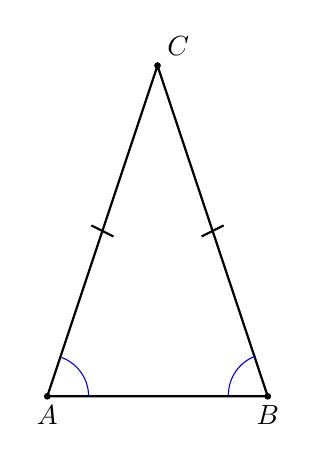
\begin{tikzpicture}[scale=0.7]
    \draw [thick](0,0)--(4,0)--(2,6)--(0,0);
    \draw [fill] (0,0) circle [radius=0.05] node[below]{$A$};
    \draw [fill] (4,0) circle [radius=0.05] node[below]{$B$};
    \draw [fill] (2,6) circle [radius=0.05] node[above right]{$C$};
    \draw [color=blue] (0,0) ++(0.75,0) arc [start angle=0, end angle=70, radius=0.75];
    \draw [color=blue] (4,0) ++(-0.22, 0.73) arc [start angle=110, end angle=180, radius=0.75];
    \draw [thick] (0.8,3.1)--(1.2,2.9); %tick mark
    \draw [thick] (2.8,2.9)--(3.2,3.1); %tick mark
    %\node [right] at (3.25,2.5){$x+7$};
    %\node [left] at (0.75,2.5){$2x+1$};
  \end{tikzpicture}
  \column{4cm}
    The two congruent angles are the \emph{base} angles. The third angle is the \emph{vertex} angle.
  \end{columns}
\end{frame}

\begin{frame}{Features of parallelograms (and rhombuses)}
  Parallelogram $SNOW$ with $S(2,1),N(7,1),O(10,5),W(5,5)$\\[0.5cm]
  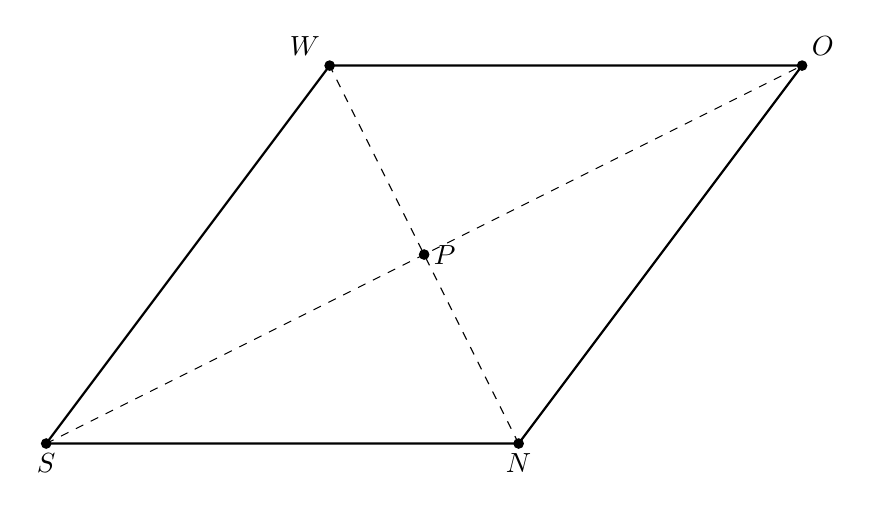
\begin{tikzpicture}[scale=1.2]
    \draw [thick] (2,1)--(7,1)--(10,5)--(5,5)--(2,1);
    \draw [dashed] (2,1)--(10,5);
    \draw [dashed] (7,1)--(5,5);
    \draw [fill] (2,1) circle [radius=0.05] node[below]{$S$};
    \draw [fill] (7,1) circle [radius=0.05] node[below]{$N$};
    \draw [fill] (10,5) circle [radius=0.05] node[above right]{$O$};
    \draw [fill] (5,5) circle [radius=0.05] node[above left]{$W$};
    \draw [fill] (6,3) circle [radius=0.05] node[right]{$P$};
  \end{tikzpicture}
\end{frame}

\begin{frame}{``SOH-CAH-TOA" trigonometric ratios}
  \begin{block}{Write in your notebook: Trig ratios, ``SOH-CAH-TOA"}
    \begin{enumerate}
        \item sine, SOH: $\displaystyle \sin x = \frac{\text{opposite}} {\text{hypotenuse}}$
        \item cosine, CAH: $\displaystyle \cos x = \frac{\text{adjacent}} {\text{hypotenuse}}$
        \item tangent, TOA: $\displaystyle \tan x = \frac{\text{opposite}} {\text{adjacent}}$
    \end{enumerate}
    \end{block}
\end{frame}


\begin{frame}{template}
  words
\end{frame}


\end{document}